\documentclass[spanish,12pt]{article}
\usepackage[spanish]{babel}
\usepackage[utf8]{inputenc}
\usepackage{xspace}
\usepackage{lmodern}
\usepackage{indentfirst}
\usepackage{xargs}
\usepackage{ifthen}
\usepackage{fancyhdr}
\usepackage{latexsym}
\usepackage{lastpage}
\usepackage{textcomp}
\usepackage{varwidth}
\usepackage{caratula, aed2-tad,aed2-symb,aed2-itef}
\usepackage{algorithmicx, algpseudocode, algorithm}
\usepackage{enumerate}
\usepackage{graphicx}
\usepackage{caption}
\usepackage{subcaption}
\usepackage{float}
\usepackage{anysize}
\marginsize{1.5cm}{1.5cm}{1.5cm}{1.5cm}

\begin{document}

\titulo{Informe 2}
\materia{Algoritmos y Estructuras de Datos III}
\author{Grupo  \\Alvarez Vico Jazm\'in\\Cortés Conde Titó Javier María\\Pedraza Marcelo \\ Rozenberg Uriel Jonathan}

\integrante {Jazmín Alvazer Vico}{75/15}{jazminalvarezvico@gmail.com}
\integrante {Marcelo Pedraza}{393/14}{marcelopedraza314@gmail.com}
\integrante {Uriel Jonathan Rozenberg}{838/12}{rozenberguriel@gmail.com}
\integrante {Javier María Cortés Conde Titó}{252/15}{javiercortescondetito@gmail.com}

\maketitle


\clearpage

\tableofcontents
\cleardoublepage

\section{Problema 1: }

\subsection{Introducción}


%terminar?%

\subsection{Explicación de la solución}


%creeeo que le falta%



\subsection{Pseudocódico}


\subsection{Demostración de Correctitud}



\subsection{Demostración de Complejidad}


\subsection{Experimentación}

%%%%%%%%%%%%%%%%%%%%%%%%%%%%%%%%%%%%%%%%%%%%%%%%%%%

\section{Problema 2: }

\subsection{Introducción}


\subsection{Explicación de la solución}



\subsubsection{Pseudocódigo}


\subsubsection{Demostración de Correctitud}


\subsubsection{Demostración de Complejidad}


\subsection{Experimentación}


\subsubsection{Análisis complejidad te\'orica}


\subsubsection{Análisis}



\section{Problema 3: Escapando}

\subsection{Introducción}

En este problema, los exploradores se encuentran en un dilema, luego de romper varias paredes la fortaleza se esta derrumbando. Por suerte ellos se encuentran en una habitación que tiene varios carritos y un mapa que les indica que estaciones estan conectadas y cuanto tardan en llegar de estación a estación. Lo que quieren es la forma más rápida de llegar desde el lugar en donde estan hasta la salida, que seria la ultima estación.

Formalmente, tenemos un digrafo rotulado, con peso en los ejes, y cada nodo esta identificado por un número desde el uno hasta la cantidad de nodos. Nuestro objetivo es encontrar el camino mínimo, dando el tiempo y su conjunto de ejes.


\subsection{Explicación de la solución}

   Inicialmente creímos que este problema podría resolverse mediante un algoritmo de BackTracking, sin embargo observamos que nunca lograríamos conseguir la complejidad pedida, puesto que este tipo de algoritmos conlleva una complejidad exponencial superior.
   Finalmente, pudimos resolverlo mediante programación dinámica. Nuestro algoritmo principal llama a dos funciones que utilizan la recursividad para poder obtener en un caso el valor óptimo, y en el otro "las mochilas llenas."
   Para facilitar el entendimiento del algoritmo introduciremos el concepto de "Hipercubo". Un hipercubo es el análogo n-dimensional de un cuadrado (n=2) o un cubo (n=3). En particular en nuestro problema tenemos un hipercubo de dimension cuatro, esta figura se denomina "teseracto", sin embargo por comodidad seguiremos llamándole hipercubo en el resto del informe.
Para poder imaginar este concepto, podríamos visualizarlo en nuestro mundo tridimencional como un vector con cubos adentro. la cantidad de cubos dependera del largo de nustra cuarta "arista".
\\
%%%%%%%%% MODIFICACION%%%%
(Por ahí nos combiene sacar lo del hipercubo, o decir que esto nos va a ayudar en la demostracion de ccomplejidad, me costo mucho explicar que representaba el hipercubo y lo pase a la versión para bobos)FIJARSE!!!!
\\
	El algoritmo se encarga de llenar un arreglo de cuatro dimensiones, donde el tamaño del arreglo principal es la cantidad de objetos y los tamaños de los otros tres arreglos anidados son las capacidades de las tres mochilas.
	Lo que representa cada posición, (x,y,z,w), de este arreglo es el valor óptimo que pueden lograr los primeros x objetos con una combinación de mochilas de peso y, z, w. En el caso que el problema a resolver responda a dos mochilas, una de las variables y, z, w seran 0 para cualquier posción y un caso similar si solo hay que llenar una mochila.
%%%%%%%TERMINA MODIFICACION%%%%
\begin{figure}[H]
\centering
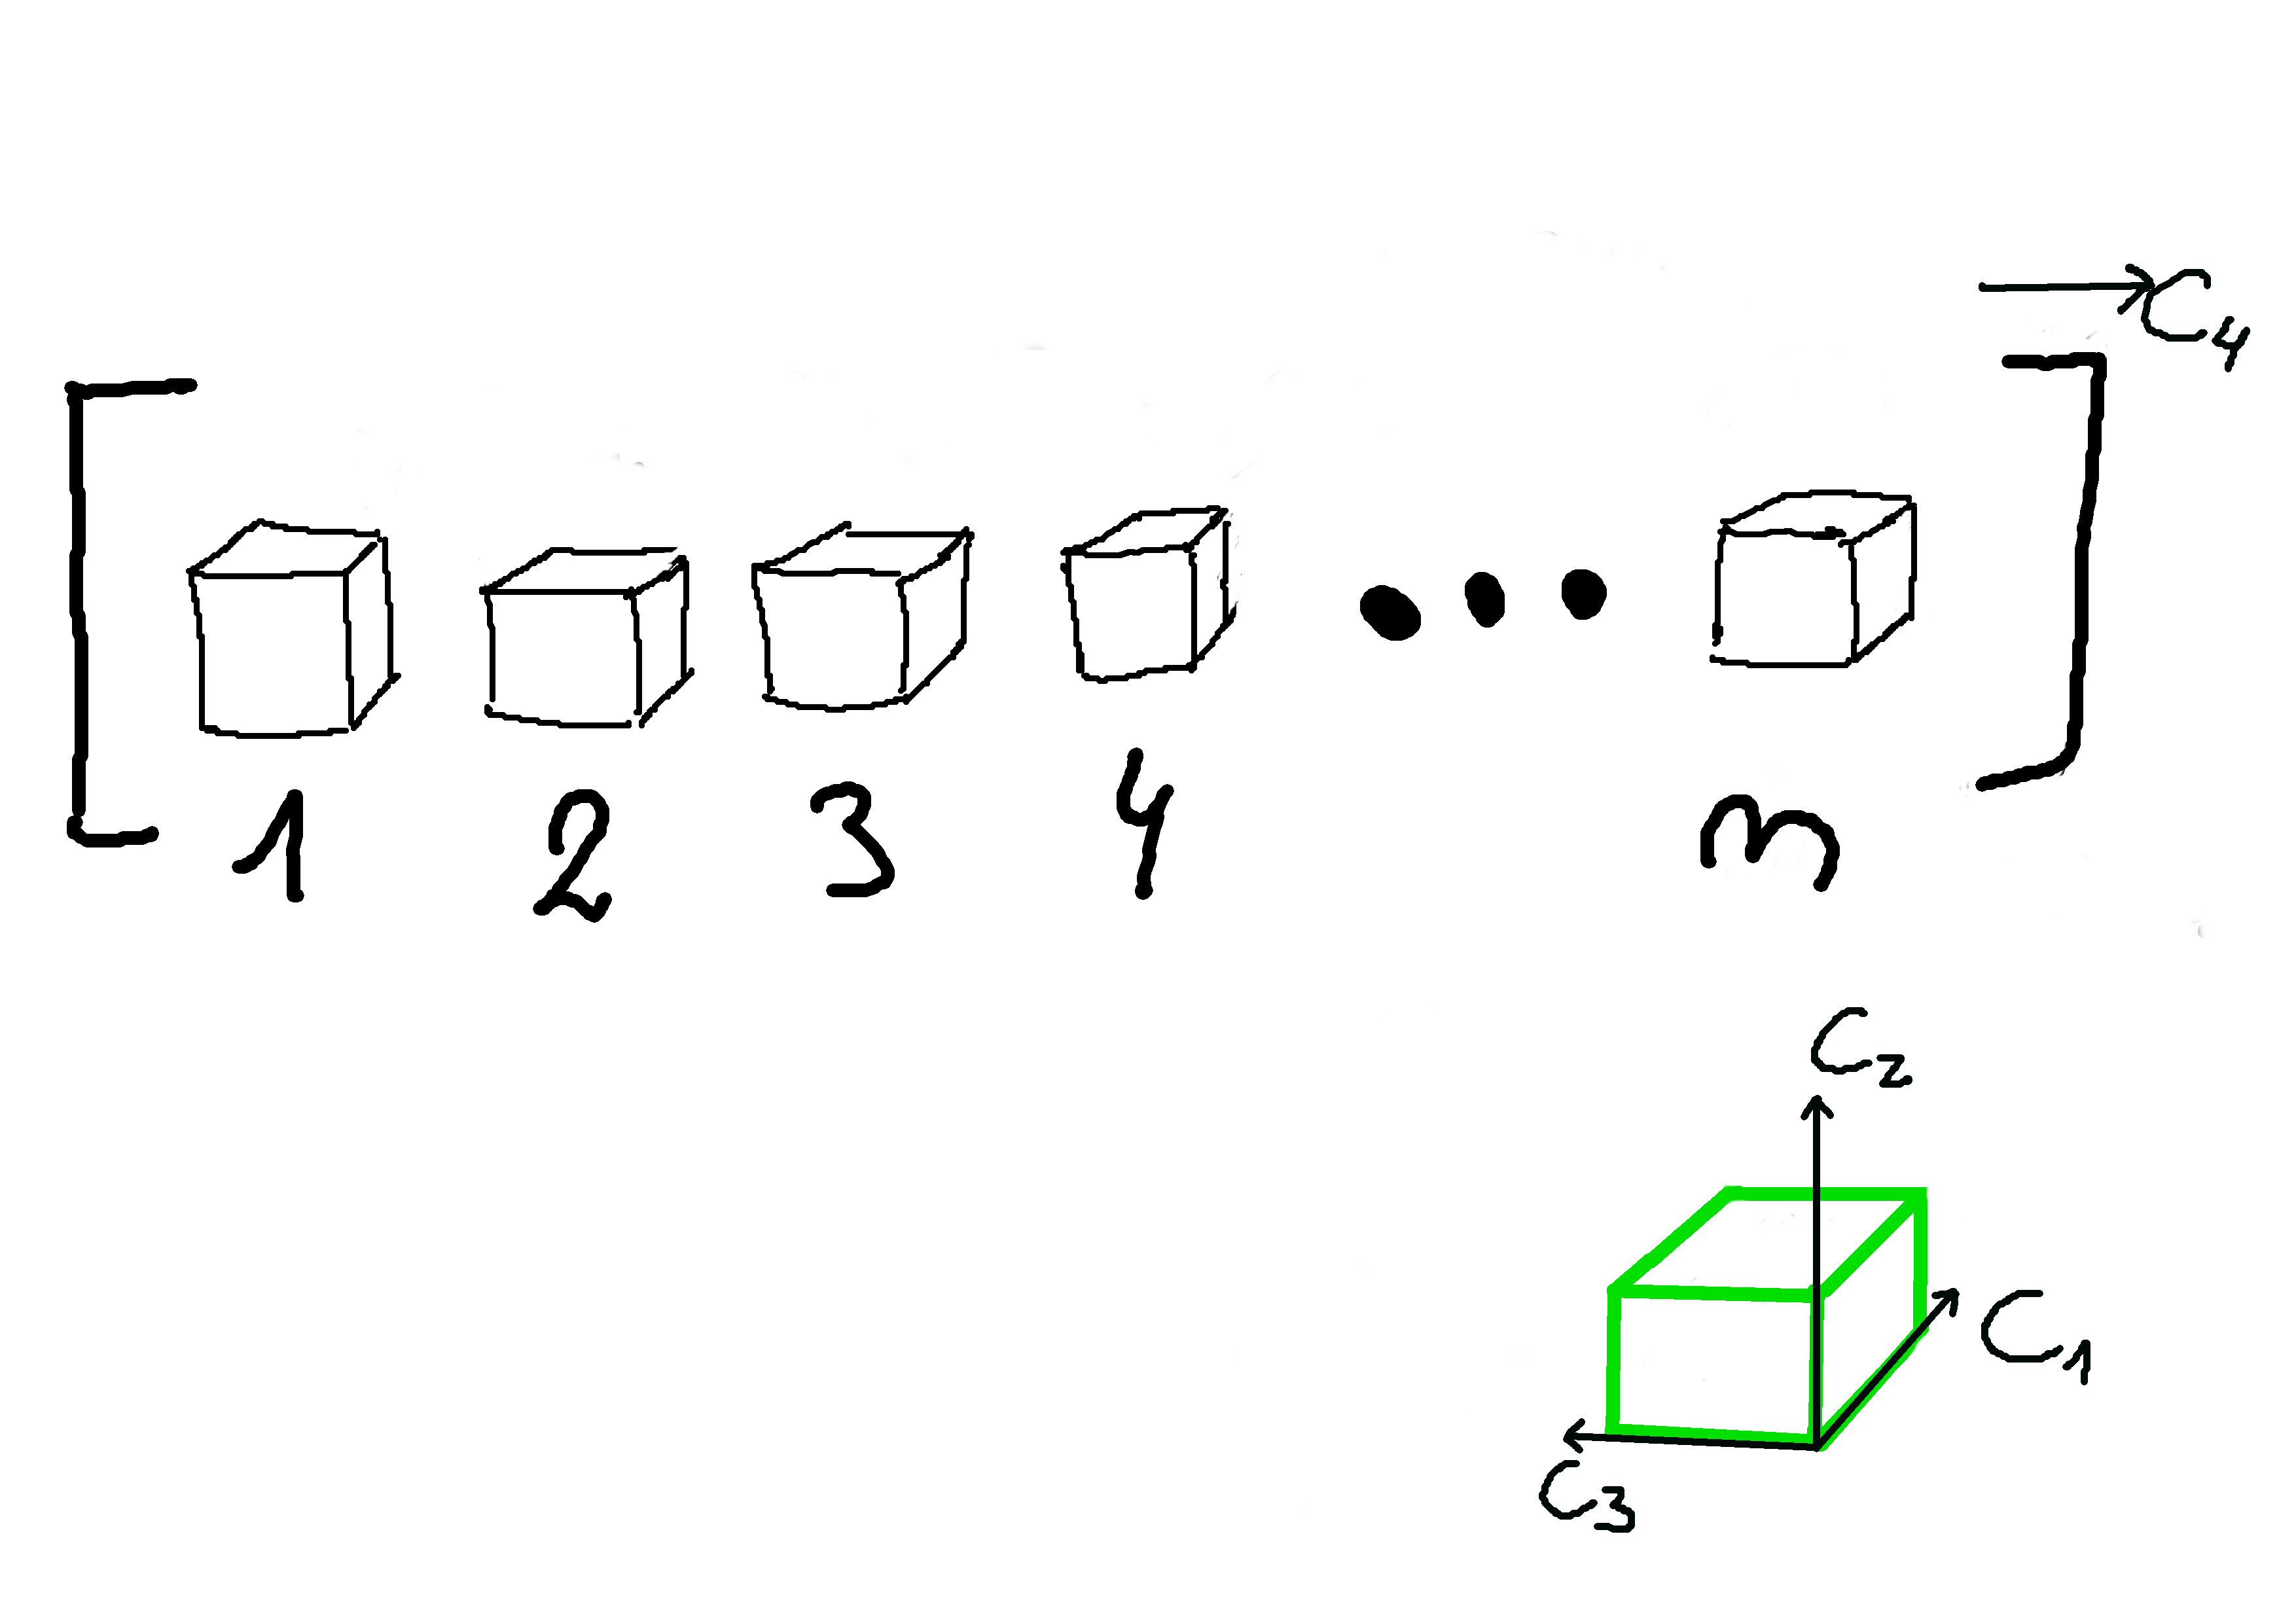
\includegraphics[width=0.4\textwidth]{hipercubo}
\caption{Imagen explicativa del concepto de hipercubo}
\end{figure}


Observación: nuestro algoritmo descarta los tesoros que tienen un peso mayor al máximo de capacidad entre las mochilas. Asumimos en el pseusocódigo que nuestra entrada cumple esa propiedad.


\subsubsection{Pseudocódigo}

\begin{algorithm}[H]{\textbf{guardandoTesoro}(mochilas: vector$<$mochila$>$, cofre: vector$<$tesoro$>$)}
	\begin{algorithmic}[1]
		%\State objXpesos $\gets$ Hipercubo() incializado en -1 \Comment (en las posiciones donde no puede haber objetos incializo en 0) %$\mathcal{O}$()
		\State objXpesos $\gets$ Hipercubo donde con todos los valores son -1 excepto en las posiciones donde no puede haber objetos que valen  0 %$\mathcal{O}$()
		\State sol$\gets$ ValorOptimo(objXpesos,cofre,cofre.size-1,capacidades de las mochilas)
		\State LlenarMochilas(objXpesos, cofre, mochila1, mochila2, mochila3)
		\State return (sol, mochilas)
	\end{algorithmic}
\end{algorithm}



\begin{algorithm}[H]{\textbf{LlenarMochilas}(objetoXpeso: hipercubo, cofre:vector$<$tesoro$>$, m1,m2,m3:mochilas)}
	\begin{algorithmic}[1]
		\State desde i= cofre.size-1 hasta i=0
			\State obj $\gets$ cofre[i]
			\State cap1 $\gets$ m1.Capacidad
			\State cap2 $\gets$ m2.Capacidad
			\State cap3 $\gets$ m3.Capacidad
			\If{$i=0$}
				\State Agregar obj en cualquier mochila en la que entre.
			\Else
				\State valM1 $\gets$ obj.valor + ValorOptimo(objetoXPeso, cofre, i,cap1-obj.peso,cap2,cap3 )
				\State valM2 $\gets$ obj.valor + ValorOptimo(objetoXPeso, cofre,i,cap1,cap2-obj.peso,cap3 )
				\State valM3 $\gets$ obj.valor + ValorOptimo(objetoXPeso, cofre,i, cap1, cap2,cap3-obj.peso )
				\State MeterEnCorrecta(valM1,valM2,valM3,m1,m2,m3,obj)
			\EndIf

	\end{algorithmic}
\end{algorithm}



%%%

\begin{algorithm}[H]{\textbf{ValorOptimo(objXpeso:hipercubo, cofre:vector$<$tesoro$>$, objeto:int, peso1: int, peso2:int, peso3:int)}}
	\begin{algorithmic}[1]
		\State  pesoObj $\gets$ cofre[objeto].peso 
		\State  pesoVal $\gets$ cofre[objeto].valor 

		\If{$peso1 < 0 \vee peso2 < 0 \vee peso3 < 0$}
			\State return $-1$ 

		\EndIf

		\If{objetoxPesos[objeto][peso1][peso2][peso3] $\neq$ -1}
			\State return objetoxPesos[objeto][peso1][peso2][peso3] 
		\EndIf
		\If{objeto $=$ 0}
			\State val $\gets$ 0 

			\If{peso1 $\ge$ pesoObj $\vee$ peso2 $\ge$ pesoObj $\vee$ peso3 $\ge$ pesoObj}
				\State val $\gets$ valorObj 

				\State objetoxPesos[objeto][peso1][peso2][peso3] $\gets$ val 
				\State return val 

			\EndIf

		\Else
			\State PosiblesSolus $\gets$ vector$<$int$>$ 
			\State sinObj $\gets$ ValorOptimo(objetoxPesos, cofre, objeto -1, peso1, peso2, peso3)
			\State PosiblesSolus.Agregar(sinObj)
			\If{peso1-pesoObj $\ge$ 0}
				\State objen1 $=$ valorObj + ValorOptimo(objetoxPesos, cofre, objeto - 1, peso1 - pesoObj, peso2, peso3)
				\State PosiblesSolus.Agrergar(objen1)
			\EndIf
			\If{peso2 - pesoObj $\ge$ 0}
				\State objen2 = valorObj + ValorOptimo(objetoxPesos, cofre, objeto - 1, peso1, peso2  - pesoObj, peso3)
				\State PosiblesSolus.Agregar(objen2)
			\EndIf
			\If{peso3-pesoObj $\ge$ 0}
				\State objen3 = valorObj + ValorOptimo(objetoxPesos, cofre, objeto - 1, peso1, peso2, peso3  - pesoObj)
				\State PosiblesSolus.Agregar(objen3)
			\EndIf
			\State valor$\gets$Max(PsiblesSolus)
			\State objetoxPesos[objeto][peso1][peso2][peso3] $\gets$ valor
			\State return valor
		\EndIf


	\end{algorithmic}
\end{algorithm}

\newpage

\subsubsection{Demostración de Correctitud}
Presentaremos la función matemática que modela nuestro problema:\\

$f(o,p_{1},p_{2},p_{3})=0 \\
f(n,p_{1},p_{2},p_{3}) = Max(V_{n}+Max(f(n-1,p_{1}-p_{n},p_{2},p_{3}), f(n-1,p_{1},p_{2}-p_{n},p_{3}), f(n-1,p_{1},p_{2},p_{3}-p_{n})),f(n-1,p_{1},p_{2},p_{3})) $
\\
Donde n representa el número de tesoro, $V_{n}$ y $P_{n}$ su valor y su peso respectivamente. $p_{1},p_{2}\ y \ p_{3}$ son las capacidades de cada mochila.

Para la demostración utilizaremos inducción global en n.
\\
\\
Caso base: queremos ver que $f(0,p_{1},p_{2},p_{3})$ resulta ser el valor máximo que se puede obtener con 0 objetos:
$f(0,p_{1},p_{2},p_{3}) = 0$ al tener 0 objetos el valor de los mismos es 0 de modo que es el máximo valor posible.
\\
\\
Hipótesis Inductiva: $\forall k<n$ vale que $f(k,p_{1},p_{2},p_{3})$ da el valor máximo que se puede obtener con k objetos.
\\
\\
Ahora queremos ver que $f(n,p_{1},p_{2},p_{3})$ da el valor óptimo para n objetos.
\\
\\
$f(n,p_{1},p_{2},p_{3}) = Max(V_{n}+Max(f(n-1,p_{1}-p_{n},p_{2},p_{3}), f(n-1,p_{1},p_{2}-p_{n},p_{3}), f(n-1,p_{1},p_{2},p_{3}-p_{n})),f(n-1,p_{1},p_{2},p_{3})) $ \\
por hipótesis inductiva (como $n-1 \leq k$ para algun k) sabemos que $f(n-1,p_{1}-p_{n},p_{2},p_{3}), f(n-1,p_{1},p_{2}-p_{n},p_{3}), f(n-1,p_{1},p_{2},p_{3}-p_{n}) y f(n-1,p_{1},p_{2},p_{3})$ son los valores óptimos que se pueden conseguir con n-1 objetos restando (o no) el peso del objeto n de modo de luego poder guardarlo en alguna mochila (o no). Utilizaremos los renombres $V_{01},V_{02},V_{03},V_{00}$ respectivamente.
Entonces tenemos: \\
$f(n,p_{1},p_{2},p_{3})= Max(V_{n}+Max(V_{01},V_{0,2},V_{03}),V_{00})$\\
Podemos ver que esta función  compara el valor óptimo de llenar las mochilas con n-1 tesoros y el tesoro n, con el valor óptimo de llenar las mochilas con n-1 tesoros sin el tesoro n (de esta forma se tiene cuenta el caso en el que el mejor valor se obtiene de poner algún objeto  de los n-1 anteriores que impide luego meter el tesoro n).\\
Como la función Max devuelve el mayor valor, el resultado sera el óptimo.
\\
Como valen P(0)..p(k) $\forall k<n$ y vale p(n) $\Rigtharrow$ vale p(n) $\forall n \in N \cup {0} $

\subsubsection{Demostración de Complejidad}

La complejidad del algoritmo GuardarTesoro es $\mathcal{O}(\prod_{i=1}^{3}K_{i} * T)$ donde $K_i$ representa la capacidad de cada mochila y T la cantidad de tesoros. Además, esta complejidad es aportada por el algoritmo ValorOptimo, entonces basaremos nuestra demostración en el mismo.

Primero haremos unas observaciones preliminares:
\begin{itemize}

	\item El volumen de un cubo es es $\prod_{i=1}^{3}A_{i}$ donde cada $A_i$ es una arista que representa el eje de la altura, el ancho o el largo. Como explicamos en la introducción gracias a nuestro modelado, sabemos que llenar una posición del cubo nos cuesta $\Theta(1)$, entonces llenarlo entero nos costará el equivalente al volumen del mismo. Podriamos visualizarlo como subdividir un cubo en cubos pequeños de dimension 1X1X1.
	\item Llenar un hipercubo con un valor determinado (como ocurre en la linea 1 de guardandoTesoro) cuesta $\mathcal{O}(\prod_{i=1}^{3}K_{i} * T)$ ya que hay T cubos para llenar.
	\item Cuando se llama a LlenarMochilas desde GuardarTesoro cuesta $\mathcal{O}(T)$ ya que en en las lineas 9,10,11 cuando se llama a ValorOptimo, el hipercubo objetoXpeso cuenta con todos lo valores ya calculados entrando en el if (linea 6) que devuelve en $\mathcal{O}(1)$ el valor.
\end{itemize}

Volviendo a la demostración, tanto en el pseudocódigo como en la función matemática podemos ver que la recursión se realiza tantas veces como la cantidad total de tesoros. Para llenar un cubo, siempre debemos recurrir al cubo anterior, uno puede pensar que esto aportaría complejidad, sin embargo, al guardar estos valores sólo construimos estos cubos una vez, y la complejidad por acceso es $\Theta(1)$.

Otra manera de verlo, es análoga a la explicación de la complejidad de llenar un cubo. Al estar llenando un hipercubo la complejidad será quivalente al hipervolumen del mismo, es decir, multiplicariamos las tres aristas anteriores por una que sería la cuarta dimensión(en este caso los tesoros).

De cualquier manera podemos concluir que la complejidad es $\mathcal{O}(\prod_{i=1}^{3}K_{i} * T)$

Ahora probemos que esta complejidad es menor a la pedida ($\mathcal{O}((\sum_{i=1}^{3}K_{i})^{3} * T)$)

$\prod_{i=1}^{3}K_{i}  = K_1*K_2*K_3$   sea $K_max = Max(K_1,K_2,K_3)$ y $K_o= K_1^3 + K_2^3 + K_3^3 - K_max^3$ entonces $K_1*K_2*K_3 < K_m^3 < K_m^3 + K_o = K_1^3+K_2^3+K_3^3 <(\sum_{i=1}^{3}K_{i})^{3}$ entonces $\prod_{i=1}^{3}K_{i}* T < \sum_{i=1}^{3}K_{i})^{3} * T $


\subsection{Experimentación}

La cota de complejidad de nuestro algoritmo es $\prod_{i=1}^{3}K_{i}* T$. Es decir que depende de la capacidad y cantidad de mochilas y la cantidad de tesoros.
En esta sección trataremos de respaldar esta cota mediante el análisis de los datos empíricos que obtuvimos a traves del testeo de nuestro algoritmo.
Con este objetivo a lo largo de los tests modificamos los inputs para observar de a una variable por vez dejando las otras constantes y así poder analizar el tiempo de ejecución en cada caso. En cada test los valores se logran al promediar un millón de iteraciones sobre el mismo input, sobre que forma tiene el input se va a hablar más adelante.
%%%%MODIFICACION "EN cada test... hablar mas adelante."

\subsubsection{Resultados y análisis}

En nuestro primer experimento fijamos una mochila con capacidad constante (50) y fuimos aumentando la cantidad de tesoros de a dos.
Así mismo, analizamos tres subcasos pertinentes: cuando los objetos están dados aleatoriamente (sin ninguna restricción sobre su peso), cuando el peso de los objetos se encuentra restringido a la capacidad de la mochila y cuando el peso de objetos es superior a la capacidad de la mochila.

\begin{figure}[H]
\centering
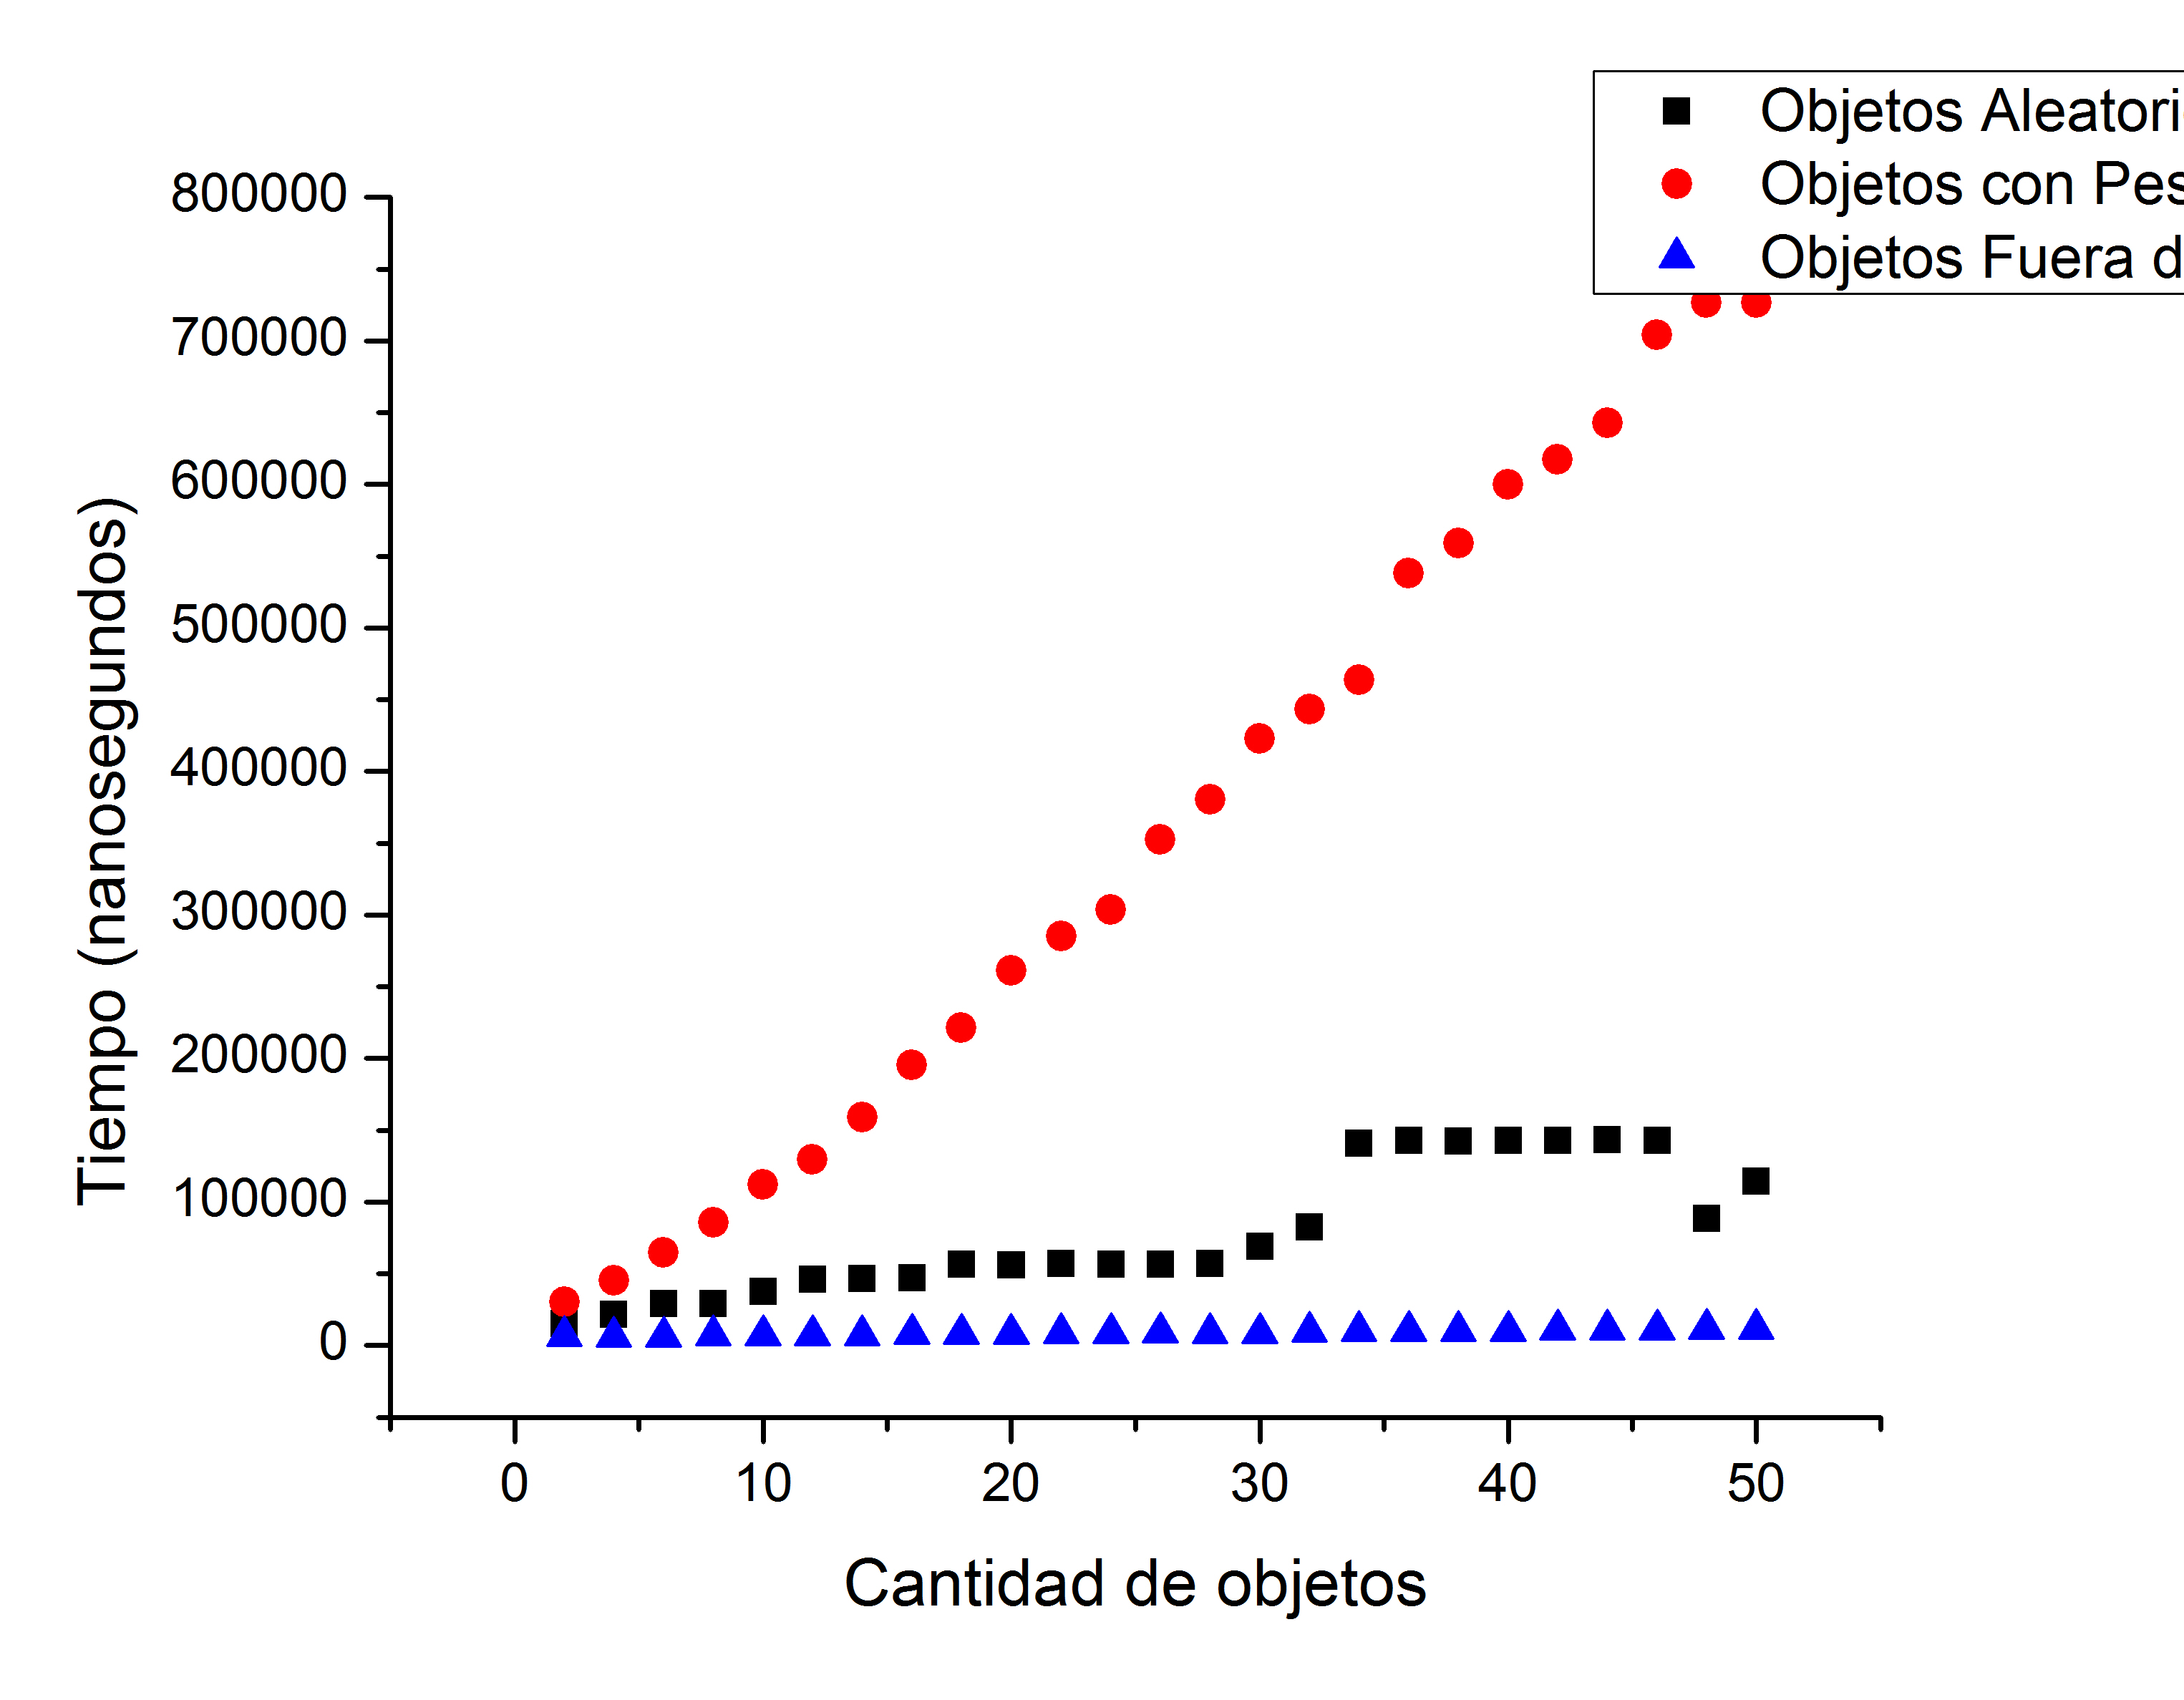
\includegraphics[width=0.6\textwidth]{comparacionObjetos}
\caption{gráfico comparativo de los tres subcasos al varias T.}
\end{figure}


En esta figura podemos observar no solo la tendencia lineal en la complejidad del algoritmo sino también la variación del crecimiento del tiempo para los distintos casos.
El hecho de que los gráficos sean lineales respaldan nuestra cota de complejidad ya que estaríamos variando el parámetro T mientras $K_1$ (la capacidad de la mochila) se mantiene constante. Estaríamos bajo la presencia de una función de tipo $Y=c*X$ con c constante.
En particular podemos destacar que en el caso de que los objetos tengan todos peso mayor a la capacidad de las mochilas, la recta tiende a ser constante y el tiempo de ejecución es casi nulo.
Podemos concluir que este sería nuestro mejor caso, y se debe al hecho de que filtramos nuestra entrada para que no se tengan en cuenta estos tesoros.
Observemos que en general lleva más tiempo obtener un resultado cuando los objetos tienen peso menor a la capacidad de la mochila.

\\
\\
\\
Luego realizamos tests para poder ver el comportamiento del algoritmo al ir aumentando el peso de la mochila. Utilizamos un test para evaluar el comportamiento cuando los objetos son aleatorios y otro para cuando todos los tesoros tienen un peso mayor a la capacidad de la mochila, en ambos casos la cantidad de objetos es constante en 50 elementos.
En esta figura podemos observar no solo la tendencia lineal de la complejidad del algoritmo sino también la variación de las pendientes en cada caso. Notemos que a mayor pendiente, la ejecución toma más tiempo, es decir es "más lenta".
En particular podemos destacar que en el caso de que los objetos tengan todos peso mayor a la capacidad de las mochilas, la recta tiende a ser constante.

\begin{figure}[H]
\centering
\includegraphics[width=0.6\textwidth]{pesoMochila}
\caption{gráfico comparativo al variar K}
\end{figure}

Podemos observar que al tener los tesoros con peso fuera del rango de la capacidad de la mochila el tiempo se mantiene constante, prácticamente nulo igual que en el experimento anterior. Con los objetos aleatorios vemos que tiene cierta tendencia lineal como es de esperarse (ya que este caso es similar al analizando en la figura()) sin embargo algunos valores quedan distorcionados. Creemos que esto se debe a que los objetos son aleatorios.
\\
\\
Finalmente corrimos tests variando la cantidad de mochilas (todas con capacidad 50) manteniendo constantes los tesoros, estos siendo 50.

\begin{figure}[H]
\centering
\includegraphics[width=0.6\textwidth]{cantMochilas}
\caption{variación de la cantidad de mochilas.}
\end{figure}

En esta figura podemos observar el crecimiento exponencial del tiempo dependiendo de la cantidad de mochilas. Esto concuerda con el hecho de que al tener todas las variables en 50 ($T=50, K_1 =50 k_2=50, k_3=50$) al ir aumentando la cantidad de mochilas estaríamos elevando la constante 50 (con $K_1$ tenemos $K_1*T=50^2$, con $K_2$ tenemos $K_1*K_2*T=50^3, etc $). Este es el tipo de función exponencial $Y=50^X$.
\\
\\
\\






:-"Y todos estos tesoros van a ir para algun museo no?"
\\
:-"Sí,Indi... lo que digas..."



\end{document}
